\documentclass[12pt,a4paper]{report}

% packages
\usepackage{CJKutf8}
\usepackage{amsmath, amsfonts, amssymb}
\usepackage{indentfirst}
\usepackage[margin=2.5cm]{geometry}
\usepackage{titlesec}
\usepackage{framed}
\usepackage{graphicx}
\usepackage{multirow} 
\usepackage{subfigure}
%\usepackage[]{mcode}

% % line spacing 

\newlength{\defbaselineskip}
\setlength{\defbaselineskip}{\baselineskip}
\newcommand{\setlinespacing}[1]{\setlength{\baselineskip}{#1 \defbaselineskip}}
\newcommand{\halfspacing}{\setlength{\baselineskip}{0.30 \defbaselineskip}}
\newcommand{\singlespacing}{\setlength{\baselineskip}{1.20 \defbaselineskip}}
\newcommand{\oneandahalfspacing}{\setlength{\baselineskip}{1.33 \defbaselineskip}}
\newcommand{\doublespacing}{\setlength{\baselineskip}{1.67 \defbaselineskip}}


\renewcommand{\arraystretch}{1.5}

% commands
\renewcommand{\arraystretch}{1.5}
\renewcommand{\figurename}{圖}
\renewcommand{\tablename}{表}
\renewcommand\contentsname{目錄}
\renewcommand\listfigurename{圖目錄}
\renewcommand\listtablename{表目錄}


\begin{document}
\begin{CJK}{UTF8}{bkai}
\titleformat{\chapter}{\Huge}{\textbf{第 \thechapter\ 章}}{1em}{\textbf}
\thispagestyle{empty}
\begin{center}
       ~\\
        \vspace{6.8cm}

        \textbf{\Huge
國立台灣大學機械工程學系 \\
系統最佳化實驗室
}
        \vspace{3cm}

        \textbf{\Huge
	Latex Basics and Text Adjustment
        }
        \vspace{6cm}

        {\large
        By  Ming-Cheng Lai
        }
        \vspace{4cm}

        {\large
            04/10/2014
        }
    \end{center}

\newpage

%\tableofcontents
%\listoffigures


\thispagestyle{empty}
~
\newpage
\clearpage
\setcounter{page}{1}
\chapter{常用的文稿類別與其中括號內的設定}

\section{類別的宣告}
\noindent\  
\LaTeX 的類別,要在文稿的一開頭時就宣告(當然,其上有註解是沒有關係的),他的一般格式如下:

		\begin{framed}
			\begin{verbatim}
			\documentclass[選擇性參數]{類別}
			\end{verbatim}
		\end{framed}
	選擇性參數是可以省略的,但類別名稱則不能省,一定要指定一個類別。而且只能只有一
個類別。


\section{類別的選擇性參數}
選擇性參數可以選擇多個,各個選項是以逗點分開的。

\begin{enumerate}
\item 10pt, 11pt, 12pt

	指定內文一般正常字的大小,預設是10pt。其他點數沒有外來package 的幫忙不能指定。

\item a4paper, letterpaper, b5paper, executivepaper, legalpaper

	指定紙張大小,預設是letterpaper。

\item fleqn 

	使數學式靠左對齊,預設是居中對齊。
\item leqno 

	使數學式編號靠左,預設是靠右。
\item titlepage, notitlepage

	決定title page 是否獨佔一頁。預設article 不獨佔一頁,但report/book 則會獨佔一頁,在這裡是可以指定來變更預設行為,例如article 文稿,指定titlepage的話,那title page 就會獨佔一頁。
\item onecolumn, twocolumn 

	文章單欄或兩欄式,預設是單欄,也就是不分欄。
\item openright, openany 

	這是在控制,章的開始是否是奇數頁(right-hand page)。在book 類別,預設章會從奇數頁開始,report 類別則不會。article 類別沒有章,所以,對此一設定會忽略。

\end{enumerate}

\section{類別的種類}
這裡只列出一般文章使用的類別,其他特殊巨集或\LaTeX 正式文件所使用的類別就不列出了,一般使用,這些類別就足夠了。

\begin {table} [h]

\centering
\begin{tabular}{| l | l | l |}
\hline

\makebox [3cm] [l] {類別} &一般用途& 特性 \\\hline
article &一般短文&無章,連續頁方式的安排,無奇偶數頁的區分\\\hline
report& 較長論文&章會起新頁,預設無奇偶數頁的區分\\\hline
book& 書籍類&章會於奇數頁起新頁,預設有偶數頁的區分\\\hline
letter &信件&英文信件格式\\\hline
slides &幻燈片&幾乎另用外來套件取代\\\hline
minimal &測試及寫新類別&這是最簡單的類別,只規定了內文的寬、高,正常字\\\hline
\end {tabular}
\end {table}


\chapter{巨集套件}
\section{\LaTeX 官方文件中的工具組}
這些巨集套件,\LaTeX 官方文件是歸類在相關軟體(relative software)中,可能會比標準巨集套件來得實用些。但也同時可以看得出來\LaTeX 非內建的套件不少,以下介紹常用的套件,一般的用法格式如下:

		\begin{framed}
			\begin{verbatim}
			\usepackage {套件}
			\end{verbatim}
		\end{framed}

\begin{enumerate}
\item  AMS-\LaTeX

\LaTeX 本身就有排版數學式子的能力,但在比較專業使用時,可能會需要增強他的功能,AMS-\LaTeX 是美國數學協會(American Mathematical Society, AMS)所發展的一個增強\LaTeX 數學式子編輯的巨集組,他主要分成兩個部份:amscls 及amsmath,前提供符合AMS 的文件規格的文稿類別,後者可加強原來\LaTeX 的數學模式。

\item graphics

這是處理圖形要用到的巨集套件。但目前一般都使用功能較完善的graphicx 巨集套件來
取代graphics 了,事實上,引用graphicx 會自動的引用graphics,而在指令使用的方便性
上,graphicx 較佳,因此我們往後都是以graphicx 為主來說明的。這兩個套件屬於LATEX
的圖形工具組,這個工具組包括了和顏色、圖形相關的各種巨集。
\item array

這是加強原來的array, tabular 環境的巨集套件,可增許多細部微調的功能。
\item dcolumn

這是讓表格中具有小數點的數字對齊的巨集套件。
\item hhline

這個巨集套件會方便在畫橫線時也可以插入表格的縱線。
\item longtable

longtable 是用在跨頁表格。通常在LATEX 中的tabular 表格是當做一個box 來處理,因此無法再分割,所以無法跨頁來表現。
\item bm

bm 的意思,就是bold math(symbol),這會讓數學式子以粗體的方式來顯示。這個巨集套
件,提供一個\verb|\bm{}| 指令,只要把數學式子置於大括號中就會由粗體來顯示。
\item enumerate

這是加強enumerate 列舉式條列環境的巨集套件。他可以很方便的指定要使用什麼方式來起頭,原始的enumerate 環境,預設第一層是阿拉伯數目字,雖然也可變更,但要重新定義,不是很方便。這裡舉個例子:
\begin{framed}
			\begin{verbatim}		
\documentclass{article}
\usepackage{enumerate}

\begin{document}
\begin{enumerate}[Example-1.]
\item This is a item 1.
\item This is a item 2.
\begin{enumerate}[(1)]
\item This is a item (1).
\item This is a item (2).
\end{enumerate}
\item This is a item 3.
\item This is a item 4.
\end{enumerate}
\end{document}\end{verbatim}
		\end{framed}
編譯後的結果如下:
\begin{figure}[!h]
\centering



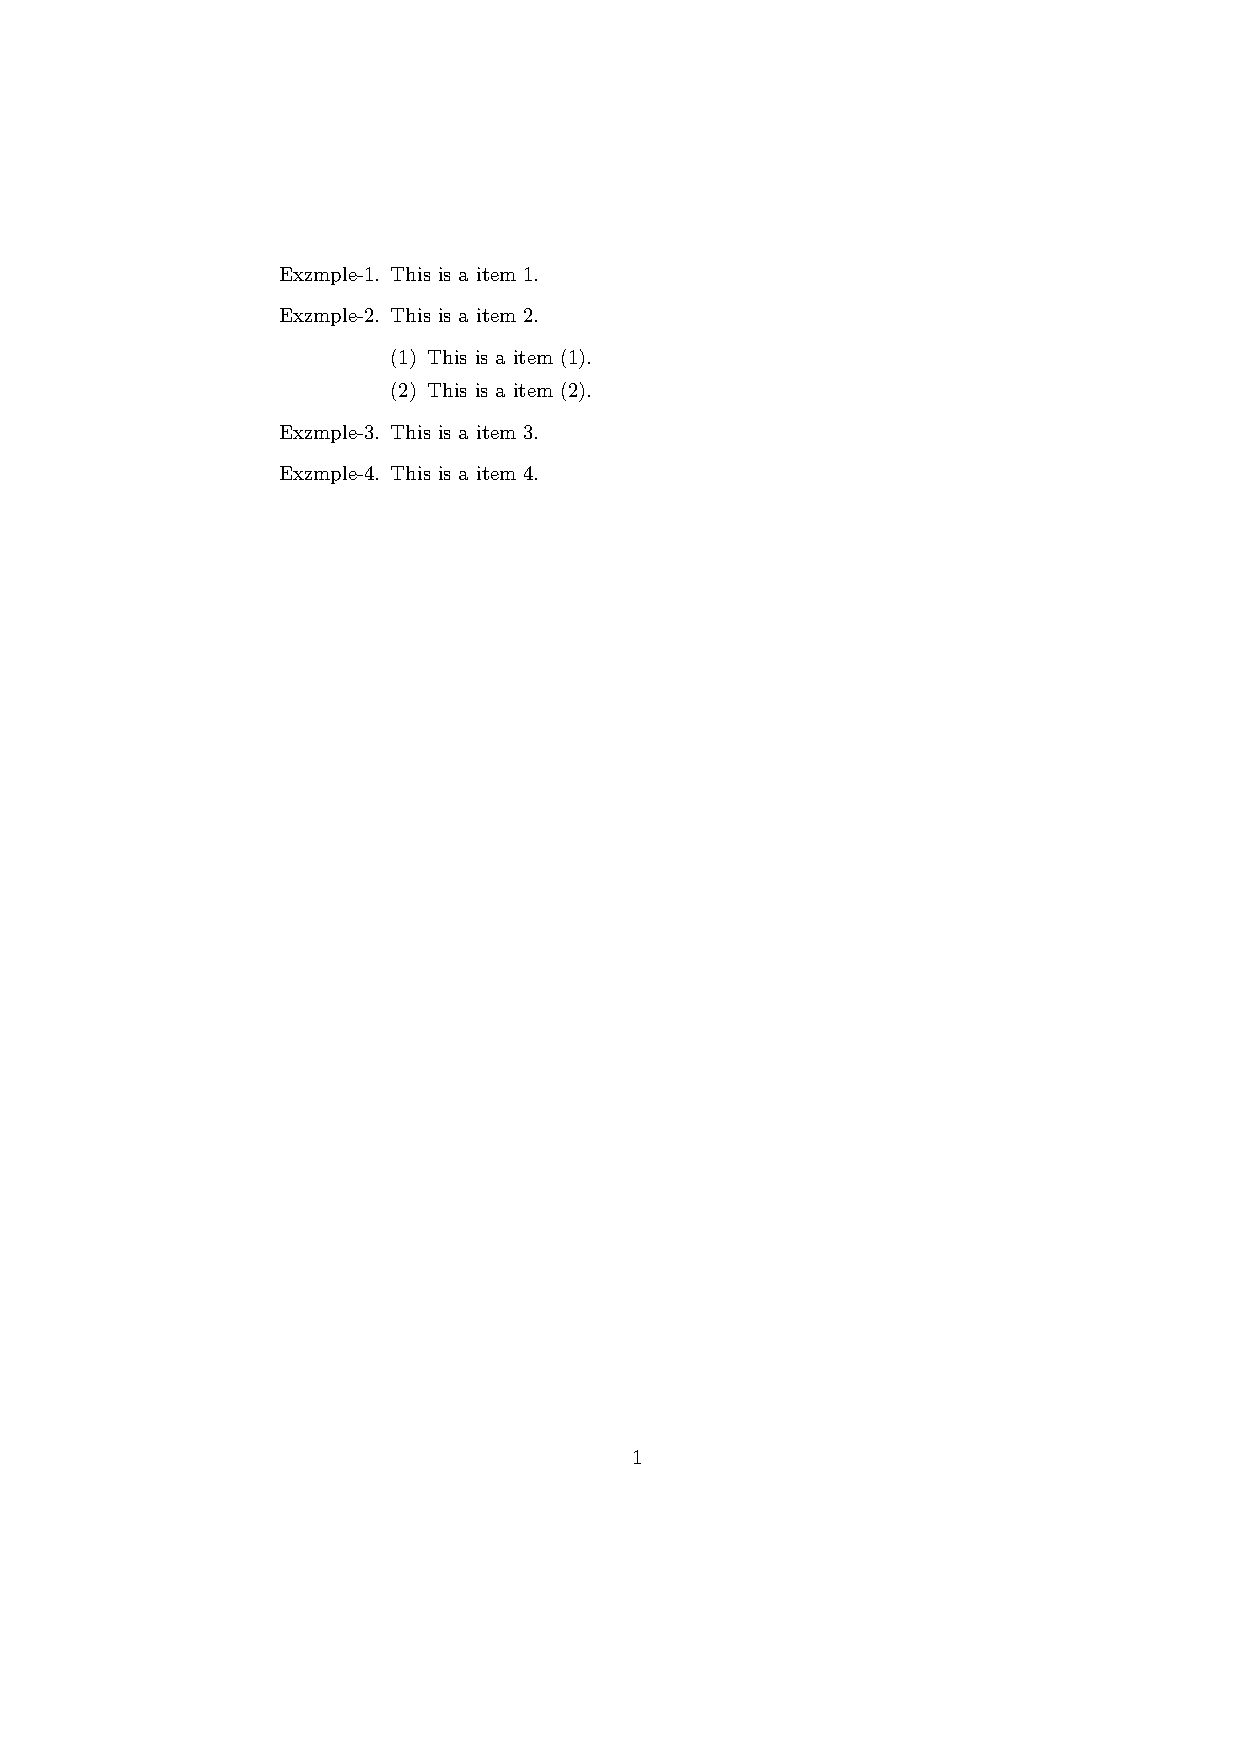
\includegraphics[trim=4.5cm 21cm 5cm 4cm,clip,scale=1]{./pics/example15}
\end{figure}

\item ftnright

\LaTeX 在兩欄式排版(two-column mode)時,他的腳註是置放在各自欄位底部。ftnright
會將兩欄式排版時,把所有的腳註都置放在右欄底部。這樣可以將腳註集中,看起來不會
那麼凌亂。
\item theorem

這是\LaTeX 內建的theorem 環境的加強型巨集套件。

\end{enumerate}


\chapter{標題以及標題頁的相關指令與用法}

這是指內頁的第一頁,我也不知道這個中文專有名詞是什麼,在\LaTeX 裡頭,我們就稱為title page。在LATEX 的標準格式裡,他包括了標題(title)、作者名字(author)、日期(date)及感謝詞(thanks)。要注意的是,在report/book 類別,title page 是自成一單獨頁的,但在article 類別裡,他是和本文連起來的。以下介紹其用法,在report/book 中:
		\begin{framed}
			\begin{verbatim}
\documentclass{report}

\title{Aesop Fables}
\author{Aesop\thanks{Thanks to the reader.}
\and Nobody\thanks{Thanks to nobody.}}
\date{\today}

\begin{document}
\maketitle
\chapter{Aesop Fables}
\section{The Ant and the Dove}
...\end{verbatim}
		\end{framed}
排版出來的結果如下:
\begin{figure}[!h]
\subfigure[page 1]{
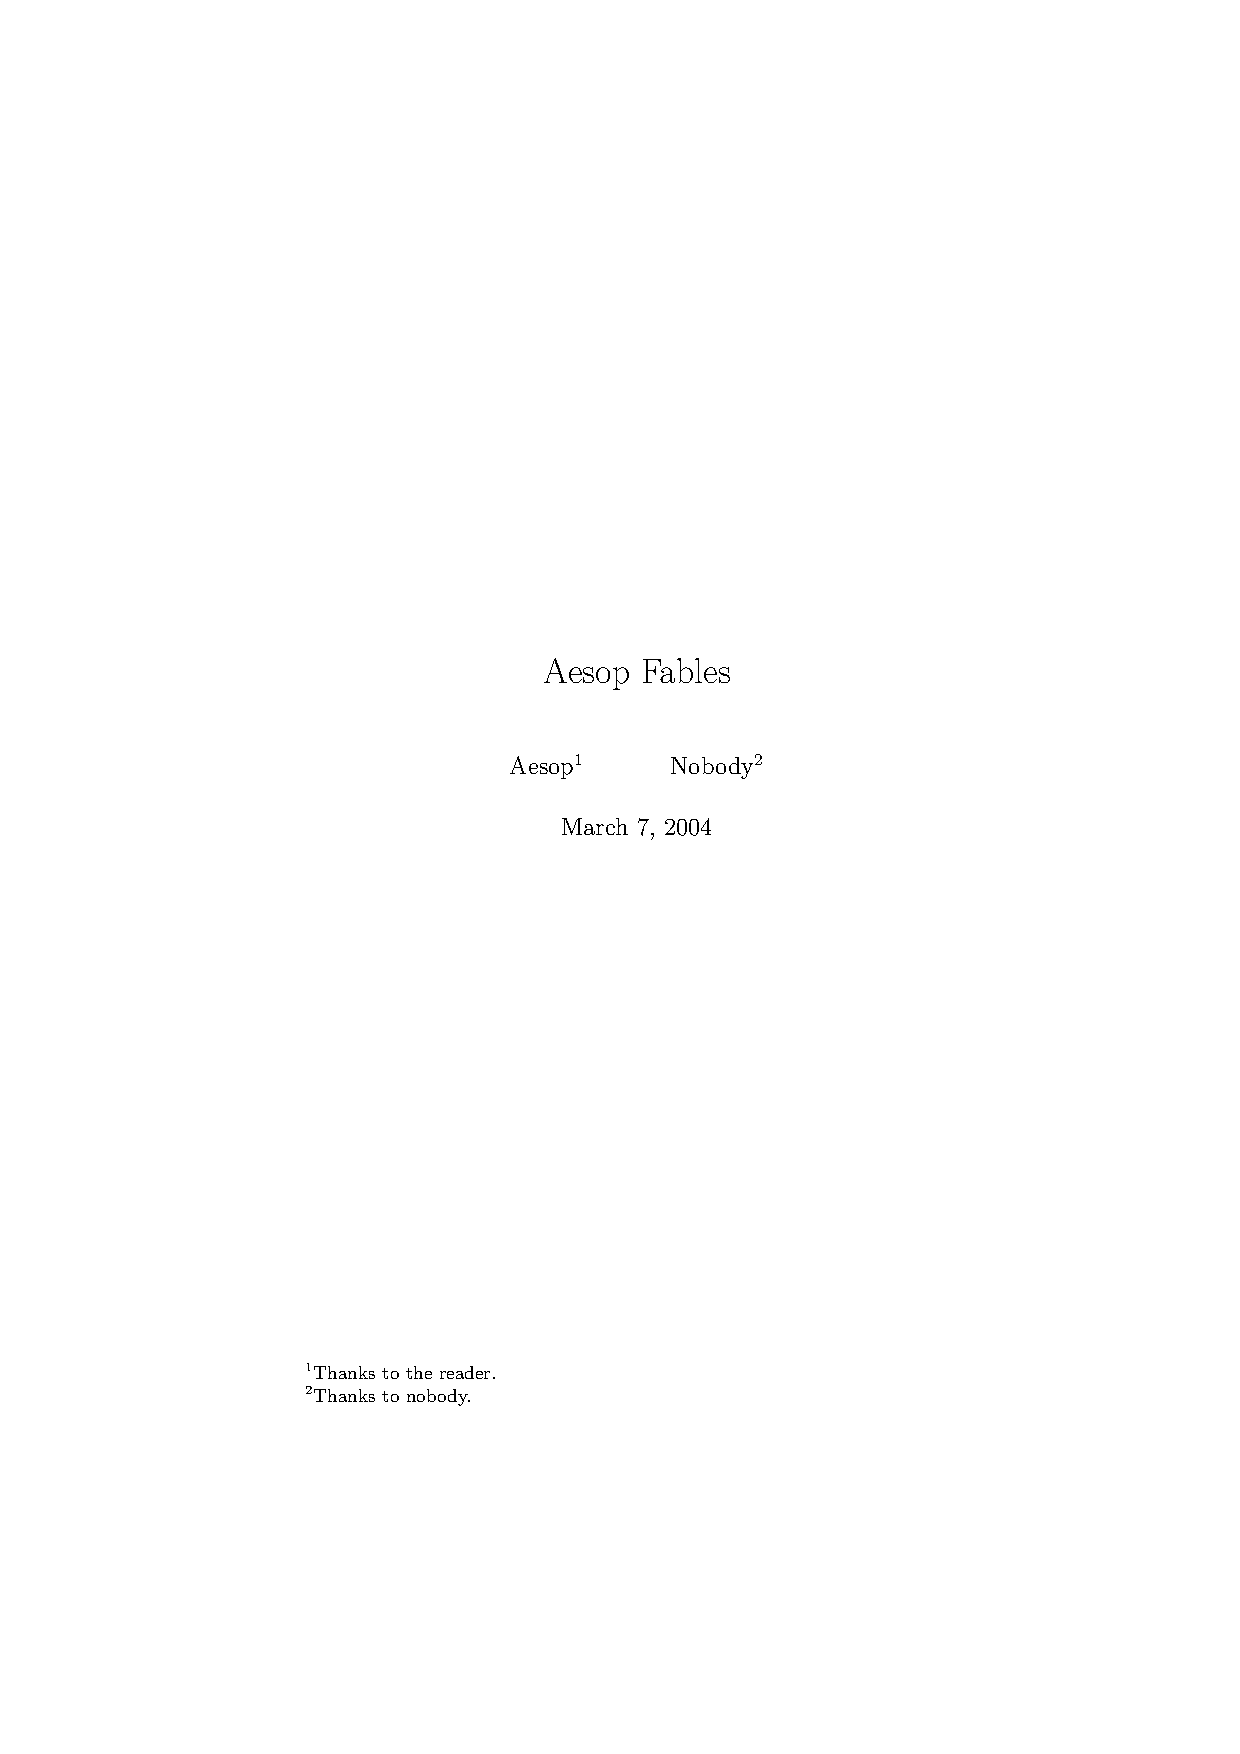
\includegraphics[scale =0.35]{./pics/1_pdfsam_example3}}
\subfigure[page 2]{
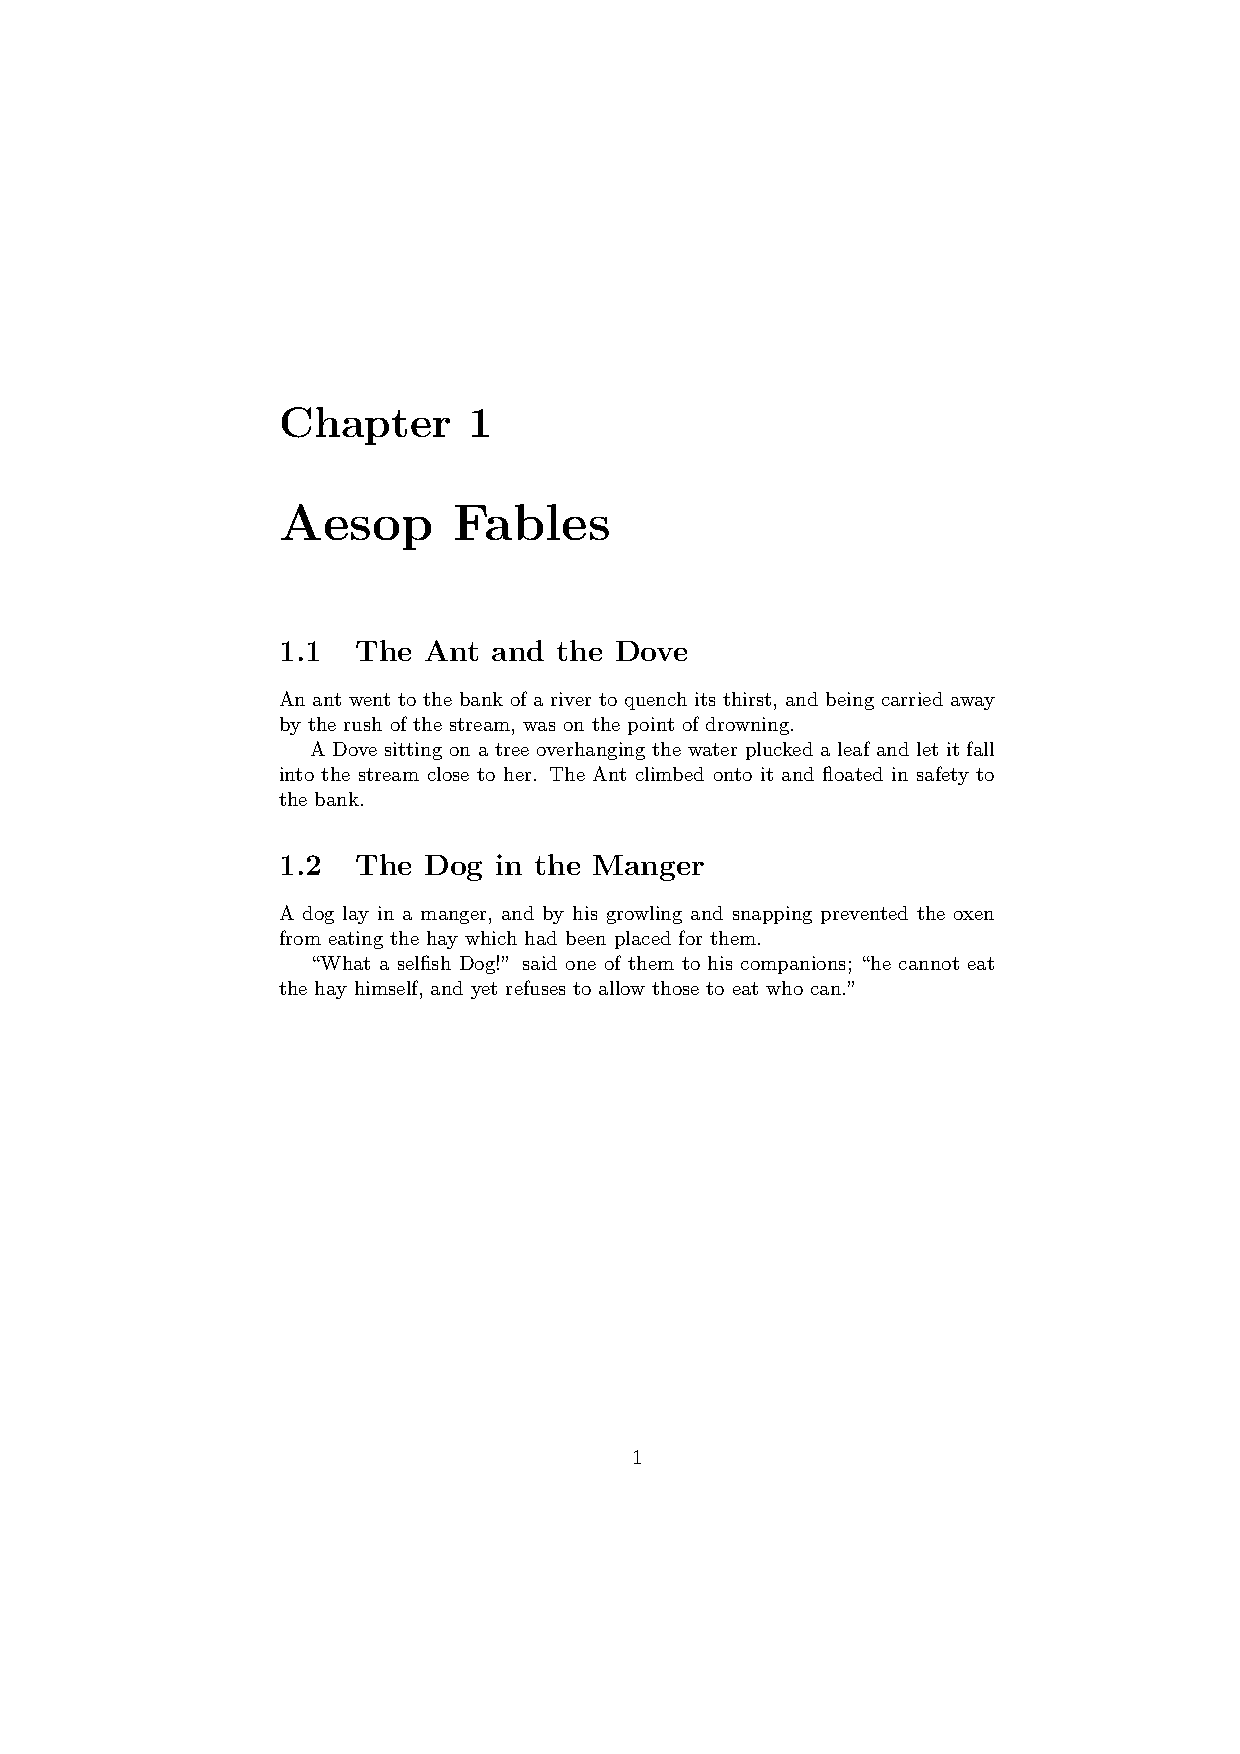
\includegraphics[scale =0.35]{./pics/2_pdfsam_example3.pdf}}
\end{figure} 

 若是在article 中:
\begin{framed}
			\begin{verbatim}
\documentclass[a4paper,12pt]{article}

\begin{document}
\begin{titlepage}
\title{The Triangulation of Titling Data in
       Non-Linear Gaussian Fashion via  Series}
\date{October 31, 475}
\author{John Doe\\ Magic Department, Richard Miles University
        \and Richard Row, \LaTeX\ Academy}
\maketitle
\end{titlepage}
This should go after the preceding commands. For
...\end{verbatim}
		\end{framed}

排版出來的結果如下:
\begin{figure}[!h]
\subfigure[page 1]{

\includegraphics[scale =0.35]{./pics/1_pdfsam_untitled-6}}
\subfigure[page 2]{

\includegraphics[scale =0.35]{./pics/2_pdfsam_untitled-6}}
\end{figure}

\chapter{設定頁面的上下左右邊界}
\LaTeX 的版面設定對初接觸的人來說,是惡名昭彰的困難、麻煩,因此這裡不多談他的設定,剛開始實在沒有必要把時間花在這個地方。如果實際想調整版面,建議使用geometry package。若各邊緣是2cm 就好,那只要在preamble 區設定:
\begin{framed}
			\begin{verbatim}
\usepackage[margin=2cm]{geometry}
\end{verbatim}
		\end{framed}

若要設定上下左右的邊界,可用以下指令:
\begin{framed}
			\begin{verbatim}
\usepackage[left=5cm, right=2cm, top=1.5cm, bottom=1.2cm]{geometry}
\end{verbatim}
		\end{framed}

\chapter{目錄、圖目錄、表目錄的使用}
目錄的問題,如果不講究的話,使用\LaTeX 預設的就行了。但如果要做調整的話,除非熟悉\LaTeX 巨集的寫法、定義,否則就得使用現成的巨集套件,例如minitoc 可讓目錄更緊湊,titletoc 更可做相當幅度的調整及美化。在\LaTeX 文稿內,\verb|\tablofcontents| 可以排版一般的章節目錄。\verb|\listoffigures| 指令以排版圖目錄,\verb|\listoftables| 指令則可排版表目錄。但圖表的話是指有進入浮動環境,使用\verb|\caption| 指令,有編號的圖表而言。請注意,這些目錄指令的置放位置會影響實際目錄出現的順序,沒有特殊需求的話,一般的順序是文、圖、表。用法如以下介紹:
\begin{framed}
			\begin{verbatim}
\documentclass[11pt]{article}
 
\begin{document}
 
\tableofcontents
\listoffigures
\listoftables
 
\clearpage
 
\section{Dummy section 1}

\begin{figure}[ht]
\begin{center}
 \caption{Dummy figure 1}
\label{fig:dum1}
\end{center}
\end{figure}
 
\begin{figure}[ht]
\begin{center}
 \caption{Dummy figure 2}
\label{fig:dum2}
\end{center}
\end{figure}
 
\begin{table}[ht]
\caption{Dummy table 1}
\begin{center}
\begin{tabular}{|c|c|}
 \end{tabular}
\end{center}
\label{tab:dum1}
\end{table}
 
\section{Dummy section 2}
 
\end{document}
\end{verbatim}
		\end{framed}

輸出結果如下:
\begin{figure}[!h]
\centering
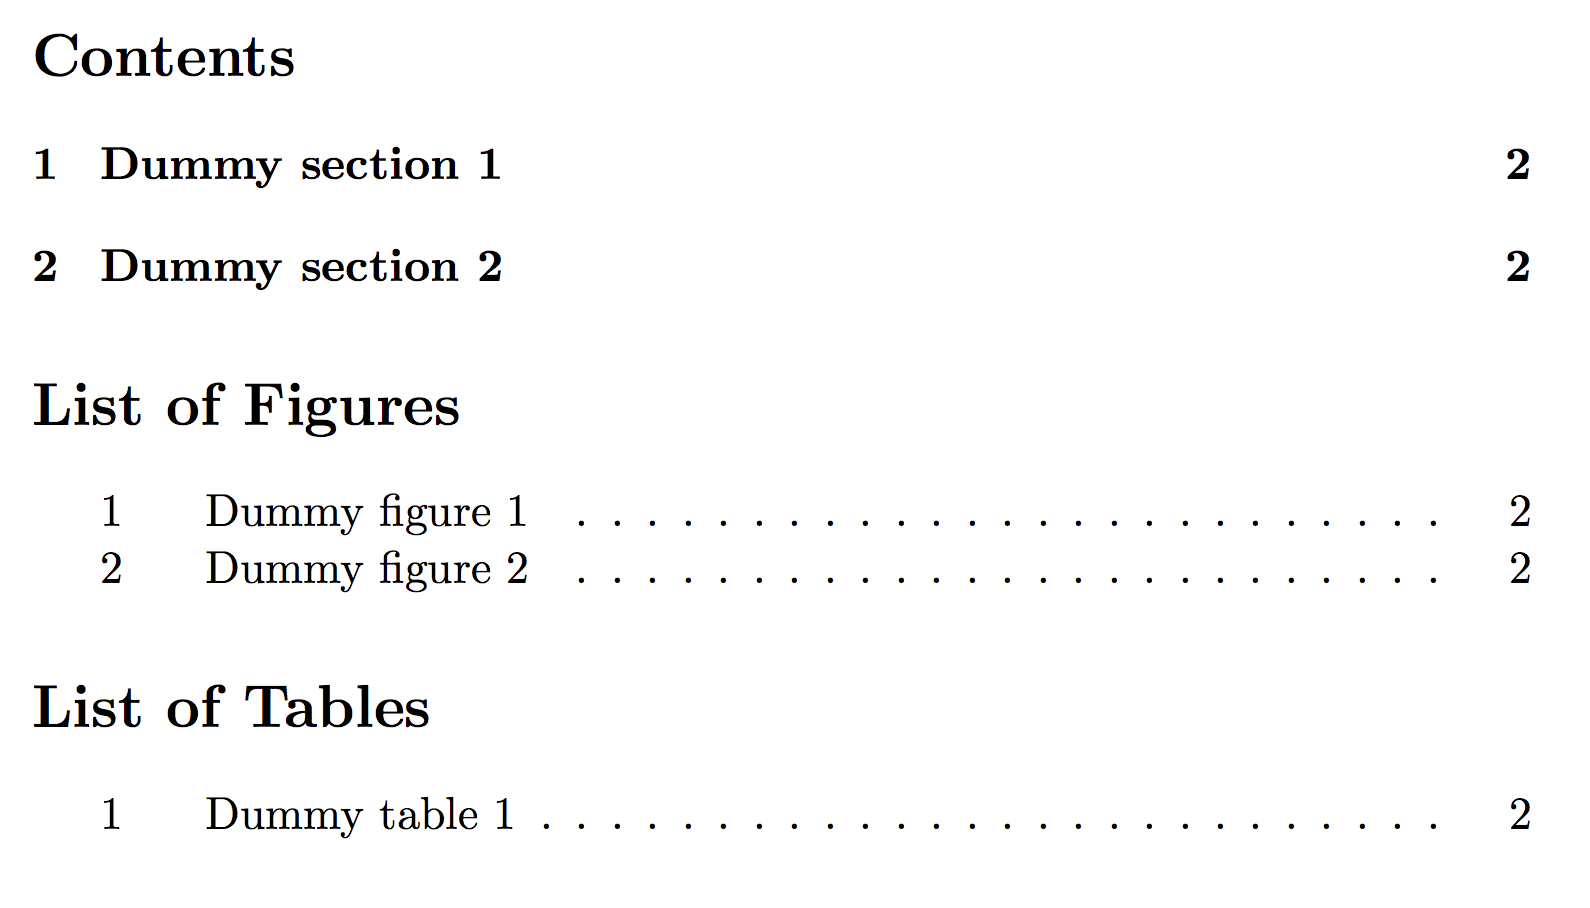
\includegraphics[scale=0.4]{./pics/simple-article-tocloflot}
\end{figure}

\chapter{設定行距}
若是對整個文件調整行距,有以下兩種方法,第一種是依照文章預設行距增加為 1.15倍(不同字型大小行距值,加大為1.15倍),在文章前面設定如下所示:
\begin{framed}
			\begin{verbatim}
\renewcommand{\baselinestretch}{1.15} 
\end{verbatim}
		\end{framed}

也可以設定絕對大小,如全部行距皆為 20 points,如下所示:
\begin{framed}
			\begin{verbatim}
\setlength{\baselineskip}{20pt}
\end{verbatim}
		\end{framed}

若改變局部行距,如局部行距變為2倍,如下所示:
\begin{framed}
			\begin{verbatim}
\usepackage{setspace}
\begin{document}
\begin{spacing}{2.0}

%行間距變為double-space

\end{spacing}
\end{document}
\end{verbatim}
		\end{framed}
\clearpage
\end{CJK}
\end{document}
